\section{The master quorum-sensing regulators LuxR/HapR directly interact with the alpha subunit of RNA polymerase to drive transcription activation in Vibrio harveyi and Vibrio cholerae}

\subsection{Нормальное название}

Главные регуляторы кворума LuxR/HapR напрямую оказывают влияние на альфа-субъединицу РНК полимеразы для управления активации транскрипции в бактериях Vibrio harveyi and Vibrio cholerae.

Quorum-sensing -- изменение поведения колонии бактерий при достижении критического значения концентрации.
\subsection{Абстракт}

В бвктериях рода Vibrio кворум контролирует экспрессию генов разных факторов группового поведения, в том числе: биолюминисценцию, формирование биопленки, вирулентность и компетентность(способность бактериальной клетки поглотить находящуюся в окружающей среде молекулу ДНК).

Основные регуляторы кворума -- это LuxR(для Vibrio harveyi)/HapR(для Vibrio cholerae) активируют экспрессию(транскрипция, трансляция, сплайсинг РНК и т.д) сотен разных генов в ответ на изменение плотности популяции. Механизм активации транскрипции факторами транскрипции TetR типа неизвестны, однако сайты связывания LuxR с ДНК, которые лежат вблизи -35 области промотера, необходимы для активации некоторых промотеров. Так, мы показали, что в Vibrio harveyi LuxR
напрямую взаимодействует с РНК полимеразой, активируя транскрипцию  биолюминисцентных генов luxCDABE.

LuxR взаимодействует с РНК полимеразой \textit{in vitro} и \textit{in vivo}, а конкретнее, с N- и C-концевыми доменами $\alpha$-субъединицы РНК полимеразы. Замены аминокислот в домене взаимодействия РНКП и LuxR уменьшают взаимодействие между LuxR и $\alpha$-субъединицей, и результатом становится возникновение дефектов активации транскрипции генов кворума \textit{in vivo}.

Домен взаимодействия РНКП и LuxR для Vibrio cholerae хранится в HapR и требуется для ативации гена hapA. Открытия, сделанные авторами статьи согласуются с моделью, в которой LuxR/HapR связываются с РНК полимеразой чтобы управлять инициацией транскрипции подмножества генов кворум-сенсинга в бактериях Vibrio.

\subsection{Картинки}

Используемый метод: \textit{in vivo} использовался метод иммунопреципитации.Заключается он в следующем: хотим понять, с чем свяжется конкретный ген LuxR. Создаем цепочки FLAG - ANTIFLAG, которые свяжутся между собой в будущем. В лабораторных условиях прикрепляем к нужному гену FLAG, пускаем его в клетку. Он связывается с какими-то частями РНКП. С помощью ANTIFLAG <<вылавлиавем>> LuxR, вместе с ним оторвется часть РНКП, с которой он успел связаться. Результаты анализируем с потмощью электрофореза.

\subsubsection{Рисунок 1}

Исследование взаимодействия LuxR и РНК-полимеразы

\begin{figure}[h]
    \centering
    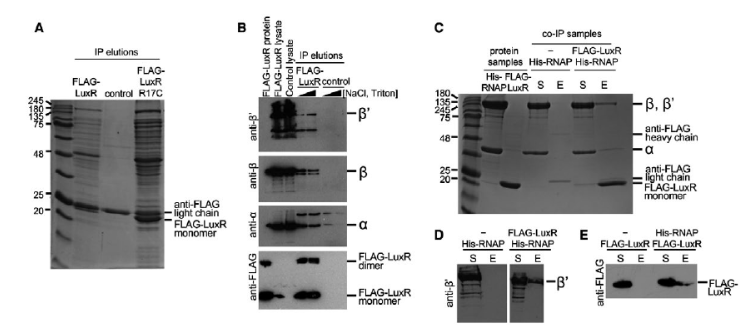
\includegraphics[width=\linewidth]{7_1.png}
    \caption{Рисунок 1}
    \label{fig:7_1}
\end{figure}

\paragraph{Рисунок 1А} 

Результаты иммунопреципитации(ИП) для оригинального гена, контрольного(без гена вообще) образца и мутанта R17C, который не умеет связываться с ДНК. В центральном столбике выделен только индикатор ANTIFLAG(очевидно, гена не было, ни с чем больше FLAG не связался). В левом столбике есть еще другие полосы, говорящие о связи LuxR с РНКП. В правом столбике темных полос много, так как в этой мутации транскрипция не могла остановиться и FLAG связался со всем подряд. 
\paragraph{Рисунок 1B}
Определение конкретных субъединиц РНКП. Здесь 2 правых столбика дублируют части рисунка 1А. Левые столбцы отражают результаты вестерн-блоттинга -- метода анализа специфичных белков. РНКП расщепляют на маленькие кусочки. Получается лизат(взвезь пептидов), который переносят на нитроцеллюлозную или PVDF-мембрану, затем детектируют с использованием антител, специфичных к заданному белку. В нерасщепленном белке(первый столбик) ожидаемо есть связь только FLAG-ANTIFLAG. Сравнение выделенных $\alpha$ и $\beta$ белков из лизата и результатов 1А позволяет определить, что с ними ген и связался изначально.

\paragraph{Рисунок 1C}
Эксперимент \textit{in vitro}.
Результаты электрофореза белков в полиакриламидном геле (перед нанесением на гель образцы кипятили в присутствии додецилсульфата натрия). His--гистидин,  хелатирует ион металла и связывается с носителем. Поскольку другие белки не связываются с носителем или связываются очень слабо, их можно удалить, промывая носитель подходящим буфером. Таким образом разделяют фазы. Столбики S -- supernatants (надосадочная жидкость), E -- элюция(то что не связалось). Таким образом \textit{in vitro} тоже подтверждает связь LuxR с $\alpha$ и $\beta$

\paragraph{Рисунки D и E}
Аналогичный рисунку 1C эксперимент, но с помощью вестерн-плоттинга. Согласуется с 1C. 
Результаты вестерн-блоттинга FLAG-LuxR и His-RNAP инкубированных с nickel-NTA resin(?). Образцы были взяты с надосадочной жидкости и элюции, вестерн-блоттинг был проведен с антителами FLAG. 

\subsubsection{Рисунок 2}
Сайты связвания LuxR с PluxC в ДНК.
\begin{figure}[h]
    \centering
    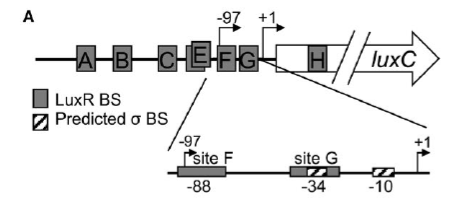
\includegraphics[width=0.7\linewidth]{7_2.png}
    \caption{Рисунок 2A}
    \label{fig:7_2}
\end{figure}

На рисунке \ref{fig:7_2} изображена диаграмма облпсть промотера гена luxCDABE. Серые квадраты отображают сайты связывания(BS), штрихованные квадраты -- предполагаемые BS. Место старта транскрипции в случае высокой плотности популяции клеток отражено черной стрелкой на +1, а низкой -- стрелкой на -97. Для кворум сенсинга основным сайтом считается +1.

\begin{wrapfigure}{r}{0.3\textwidth}
  \begin{center}
    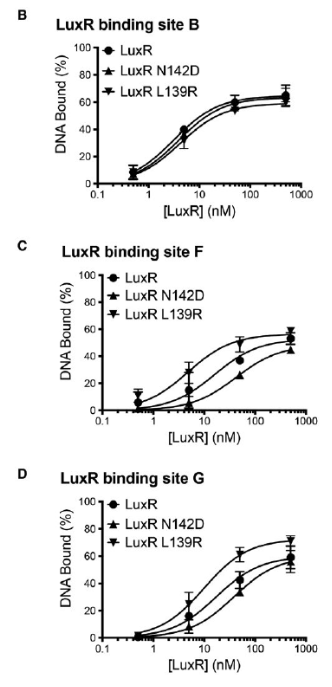
\includegraphics[width=0.28\textwidth]{7_3.png}
  \end{center}
  \caption{Рисунок 2B, C, D}
  \label{fig:7_3}
\end{wrapfigure}
Эксперименты по сдвигу подвижности были проведены с dsDNA субстратами для разных сайтов LuxR (рис. \ref{fig:7_3}). Было проведено сравнение LuxR, LuxR N142D и LuxR L139R в зависимости от концентрации. Процент связи с ДНК отражается на вертикальной оси.
Сайты связывания A-G все необходимы для активации транскрипции. Ближе всех к предполагаемому месту начала транскрипции при высокой плотности клеток находится сайт G, а низкой -- сайт F. 

Так как F и G сайты являлись кандидатами для места посадки LuxR, авторы статьи сравнили силу связи  в них и в относительно далеком сайте B.

(я в этом не уверена)
Возможно, из-за того что для разных мутаций белка значительнее различались результаты электрофореза на последних двух графиках, был сделан вывод о том, что LuxR крепится близко сайтам F и G.

\subsubsection{Рисунок 5}

На рисунке \ref{fig:7_4}A изображена структура белка Vibrio vulnificus SmcR. Красным отмечены разные аминокислоты, которые предположительно связываются с ДНК. 

На рисунке B изображен график интенсивности биолюминисценции в зависимости от того, какую из аминокислот, отмеченных на рисунке А заменили на мутирующую. Видно, что некоторые замены не оказали влияния в сравнении с оригинальным (немутантным) образцом (WT), в то время как другие не дали инициироваться процессу люминисценции.

Примечание: $OD_{600}$ это оптическая плотность, мера ослабления света прозрачными объектами или отражения света непрозрачными объектами. Вычисляется как десятичный логарифм отношения потока излучения падающего на объект, к потоку излучения прошедшего через него, то есть это есть логарифм от величины, обратной к коэффициенту пропускания.

\begin{figure}
    \centering
    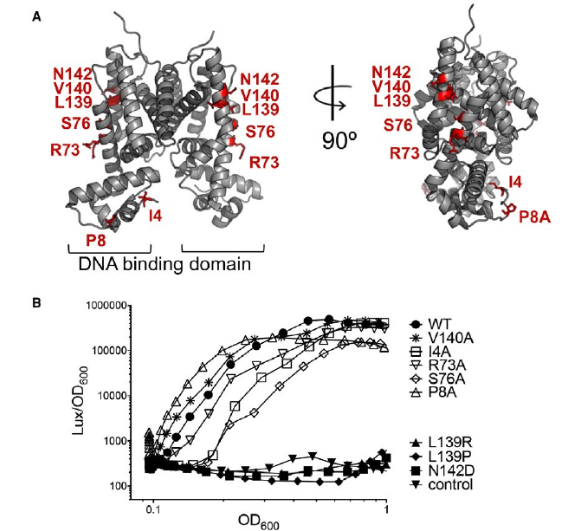
\includegraphics{7_4.png}
    \caption{Caption}
    \label{fig:7_4}
\end{figure}

\subsubsection{Рисунок 6}

На рисунке \ref{fig:7_6}A отображено выравнивание доменов взаимодействия с РНАП для разных белков (бактерия Vibrio cholerae). Черные треугольники указывают на положение аминокислот. 

На рисунке \ref{fig:7_6}B сравнивается биолюминисценция контрольного (немутантного) образца $\Delta$hapR(a), пустой последовательности(b)

Продуцирование биолюминесценции продемонстрировало значительное снижениеу штаммов, экспрессирующих hapR S77A и N143D и была полностью прекращена в штамме, экспрессирующем ДНК-связывающий мутант hapR R18C. 

Значит, поскольку эти замены в HapR приводят к фенотипам, сходным с аналогичными заменами в домене взаимодействия РНК-полимеразы LuxR,  HapR взаимодействует с РНК-полимеразой через тот же домен взаимодействия, что и LuxR. 


\begin{figure}
    \centering
    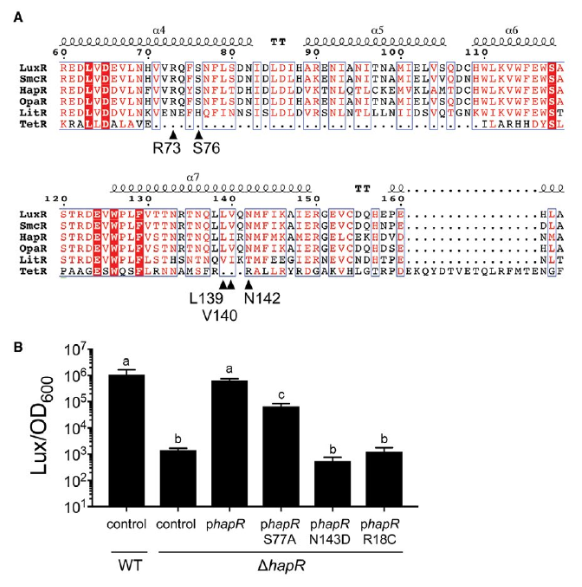
\includegraphics{7_6.png}
    \caption{Рисунок 6}
    \label{fig:7_6}
\end{figure}

\subsubsection{Рисунок 7}

Модель взаимодействия LuxR с РНКП на промотере luxCDABE. LuxR связывается с сайтами F и G, которые находятся на -88 и -34 относительно старта транскрипции (указан черной стрелкой). LuxR связывается с РНКП через взаимодействие с $\alpha$субъединицей, C-концевым доменом (сайты F и G) and N- (сайт G). Предполагаемые сайты взаимодействи обозначены черными кругами. Сайт связи LuxR и G расположен на -35 сайте для $\sigma^{70}$.

Сигма-фактор - это белок, необходимый для инициации транскрипции у бактерий. Это бактериальный фактор инициации транскрипции, который обеспечивает специфическое связывание РНК-полимеразы (RNAP) с промоторами генов.
\begin{figure}
    \centering
    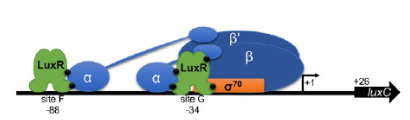
\includegraphics{7_7.png}
    \caption{Рисунок 7}
    \label{fig:7_7}
\end{figure}